\documentclass{beamer}



\mode<presentation> {
    \usetheme{Alife}
}

%\nonumberslides % descomentar para no numerar las diapositivas

% Comentar el campo que no desea que aparezca
\infopresentation[
    title = {(Title of the Presentation)},
    shorttitle = {(Short title of the Presentation)},
    subtitle = {(Subtitle of the Presentation)},
    author = {Author: (Name)},
    emailauthor = {(prefix)@unal.edu.co},          
    advisor = {Advisor: Jonatan Gómez Perdomo, Ph.D.},
    emailadvisor = {jgomezpe@unal.edu.co},
	coadvisor = {Coadvisor: Rodrigo De Castro Korgi, Ph.D.},
    emailcoadvisor = {rdecastrok@unal.edu.co },
    shortauthor = {(Name) \& J. Gómez},
    program = {(Doctorate/Master) in Computer Engineering},
    group = {Research Group on Artificial Life -- Grupo de 
            investigación en vida artificial -- (Alife)},
    department = {Computer and System Department},
    school = {Engineering School},
    institute = {Universidad Nacional de Colombia},
    shortinstitute = {UN},
    date  = {(1st Semester 2017)},
    logogroup = {images/logoALIFEcolor.pdf},
    logoinst = {images/Escudo_unal_2016.png},
    subject = {presentation ALIFE Group}
]

\AtBeginSection
{%
\begin{frame}<beamer>{Outline}%esquema
\tableofcontents[currentsection]%,currentsubsection
\end{frame}
}

%\AtBeginSubsection
%{%
%\begin{frame}<beamer>
%\frametitle{Contents} \tableofcontents[currentsection,currentsubsection]
%\end{frame}
%}

%\beamerdefaultoverlayspecification{<+->}

\theoremstyle{definition}
    %\newtheorem{definition}{Definition}
    \newtheorem{definitionc}{Definition (continuation)}
    %\newtheorem{definitions}{Definitions}
    \newtheorem{specification}{Specification}
    %\newtheorem{example}{Example}
    \newtheorem{examplec}{Example (continuation)}
    %\newtheorem{examples}{Examples}
\theoremstyle{theorem}
    \newtheorem{proposition}{Proposition}
    %\newtheorem{theorem}{Theorem}
    \newtheorem{theoremc}{Theorem (continuation)}
    \newtheorem{thesis}{Thesis}
    %\newtheorem{lemma}{Lemma}
    %\newtheorem{corollary}{Corollary}
    %\newtheorem*{proof}{Proof}
    \newtheorem*{proofc}{Proof (continuation)}
\theoremstyle{remark}
    \newtheorem*{remark}{Remark}
    %\newtheorem*{note}{Note}
    \newtheorem*{notes}{Notes}

\begin{document}
\renewcommand{\tablename}{Table}
\renewcommand{\figurename}{\scriptsize Figure}

\begin{frame}{Inicio}
\begin{center}
    Agentes Inteligentes \\
    Capítulo 2
\end{center}
\end{frame}

\begin{frame}{Recordatorios}
Tarea 0 (Actualización lisp) para 28/01 \\
Tutorial Lisp/emacs/AIMA: 11-1 hoy y lunes, 271 soda

\end{frame}

\begin{frame}{Agentes basados en utilidad}
  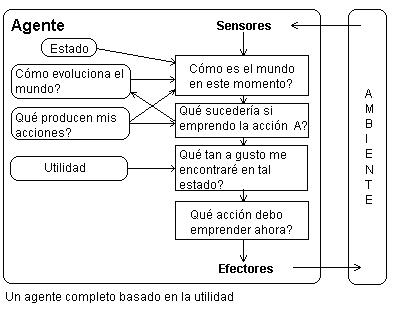
\includegraphics[width=\textwidth,height=\textheight,keepaspectratio]{25_utilidad.jpg} 
  % (tomado de https://sites.google.com/site/inteligenciaartificial8avo/agentes-inteligentes/agentes-basados-en-utilidad)
\end{frame}

\begin{frame}{Agentes que aprenden}
  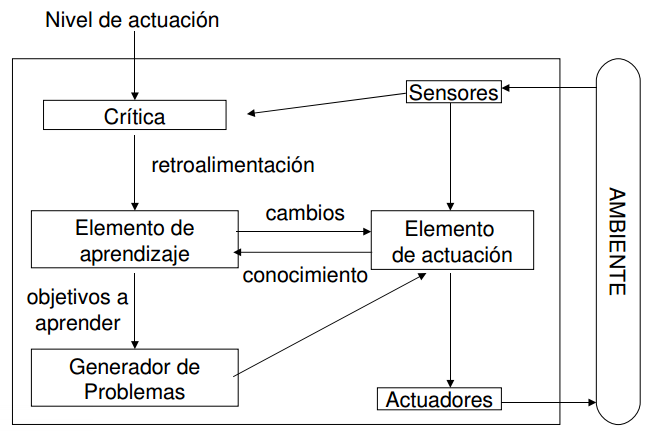
\includegraphics[width=\textwidth,height=\textheight,keepaspectratio]{26_queaprende.png}
  % (tomado de https://freedoomforlife.wordpress.com/agentes/)
\end{frame}



\end{document} 
